\documentclass[a4paper]{article}

\usepackage[utf8]{inputenc}
\usepackage[margin=0.8in]{geometry}

\usepackage{rotating, graphicx}
\graphicspath{ {../} }
	
\begin{document}


\title{Real World Idris \\ Project Scope and Outline}
\author{Ioan Luca \\ \small 201638554}
\date{\today}
\maketitle


% Your submission needs to include the code (zipped up) along with a short report (I'm only after a few pages) by which includes:

% An overview of the chosen problem(s).
% An outline of your solution and a high-level overview of your
% design (a class diagram is fine - just an indication of who you have structured your solution)

% Details of any important/interesting parts of your implementation.
% Results and evaluation - what it does and how well it does it. You should run your solution over the entire test system provided and summarise the outputs in terms of: a) which smells were accurately detected, b) which were missed, and c) what false positives (incorrectly flagged up by your system as smells) were identified. It is likely that will be the majority of the report.

% A statement of the score (out of 20) that you think the work deserves along with a short justification for this (a couple of sentences).


% You
% will also be required to demonstrate your system in week 6/7.Additional Information on the marking schemeThere
% are three basic components to how your submission will be assessed:
% what it does, how well it does it, and how you went about doing it.

% What it does: Some tasks are more complicated than others (see the table above)

% How well it does it: This ranges from brilliantly - produces the
% correct results for all the time, to adequate - works
% reasonably well for a limited number of cases, to... well let's not aim for that.

% How you went about doing it: This considers what facilities of the JavaParser framework
% you employed and also also the quality of your design.

\section{Code Smells Overview}
I attempted the ''Middle Man'' code smell from the Hard category,
the ''Long Method'', ''Switch Statements'' and ''Primitive Obsession'' code smells
from the Medium category as well as
the ''Long Class'' and 'Long Parameter List'' from the Easy category.

\subsection{Middle Man}
This code smell happens when a class delegates all of its responsibility to
another class, usually when attempting to reduce high coupling. However, this
way it essentially becomes useless.

The software identifies such behaviour by using 2 visitors.
The first one traverses all the methods in scope to compile a set of all the
method names.
The second visitor identifies methods with a single statement or with 2
statements
out of which the outer one is a return.
If the statement is a method call that is part of the list, then the smell was
found.

\subsection{Long Method and Long Class}
Long methods/classes are a sign of bad incremental design.
Functionality has been
extended over time without taking into account refactoring.
They are hard to read and they usually denote breaking of the
''Single responsibility principle''.
The software detects such methods/classes by counting the statements inside its
body, including arbitrarily nested statements.
If the number exceeds 10/100, the smell was found.

\subsection{Switch Statements}
Switching on type codes is a bad practice in OOP and it should be handled by
subclassing.
This code is detected when the expressions being switched on is of
a user defined Enum type.

\subsection{Primitive Obsession}
This appears when sufficiently complex data is handled by primitive types
instead of being abstracted away in a class.
It favours the birth of Data Clumps smells as well.
The software detects this smell inside method declarations and classes by
counting all the total number of variables, parameters and fields.
Then, the primitive declarations are selected from the total and ratio
is calculated with $ratio=\frac{primitives}{total}$.
If $ratio \geq 0.37$ and $primitive \geq 4$ then the code smell was discovered.
The numbers came from a lot of trial and error and they seem to discover this
code smell wherever it is present in the testing system.

\subsection{Long Parameter List}
Similar to the Primitive Obsession, having too many parameters breaks both
encapsulation and abstraction and.
In addition, such a code smell provides a clear clue that the implementation
of the method is quite complex.
The software detects parameters lists for both methods and constructors
with more than 5 parameters.

\section{High-level design}

\begin{sidewaysfigure}
	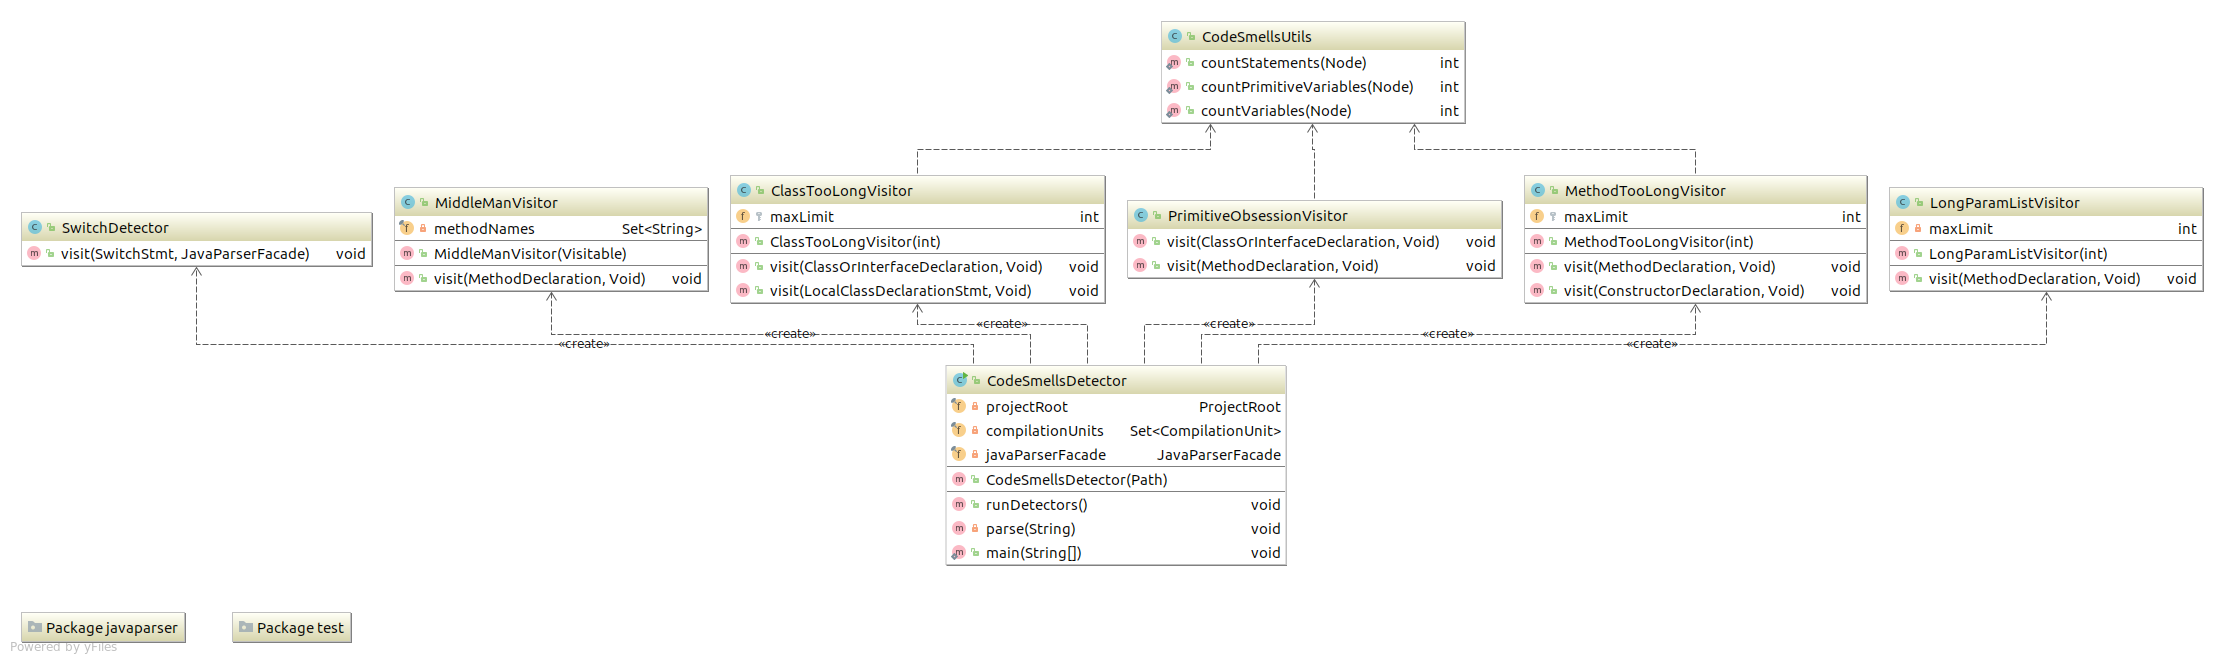
\includegraphics[width=\textwidth]{codesmellspng}
	\caption{Each code smell is implemented using a visitor that extends either
		the generic JavaParser visitor or the the void one.
		The CodeSmellsDetector class is responsible for loading and parsing all
		the sources found in the test system.
		It also runs each visitor on compilation units and
		groups errors by classes.
		Finally, CodeSmellsUtil provides useful functions like counting
		nested statements.}
\end{sidewaysfigure}

Each code smell is implemented using a visitor that extends either
the generic JavaParser visitor or the the void one.

The CodeSmellsDetector class is responsible for loading and parsing all
the sources found in the test system.
It also runs each visitor on compilation units and
groups errors by classes.
Finally, CodeSmellsUtil provides useful functionality like counting
nested statements



\pagenumbering{arabic}
\end{document}
